\chapter{Literature Review}\label{cha:literature}

    TODO: Some other intro

\section{State of the Art}

    TODO: some intro

    \subsection{ROS on Web}

        The closest representation of the intended project is the work produced by Michael Allwright known as \textit{ROS on Web}. Allwright shares the same goal as the author to develop the technology which allows for running ROS nodes entirely on the browser by cross-compiling C++ code to WebAssembly and using web workers to handle the internal communication~\cite{rosonweb}.

        Equivalently, Allwright targeted the \ac{ROS} 2 distribution. It is suspected that the \textit{galactic} version was used for the demonstrations. The main demonstration of a running publisher and subscriber is illustrated in Figure~\ref{fig:rosonweb}.
        
        
        \begin{figure}[htbp]
            \centering
            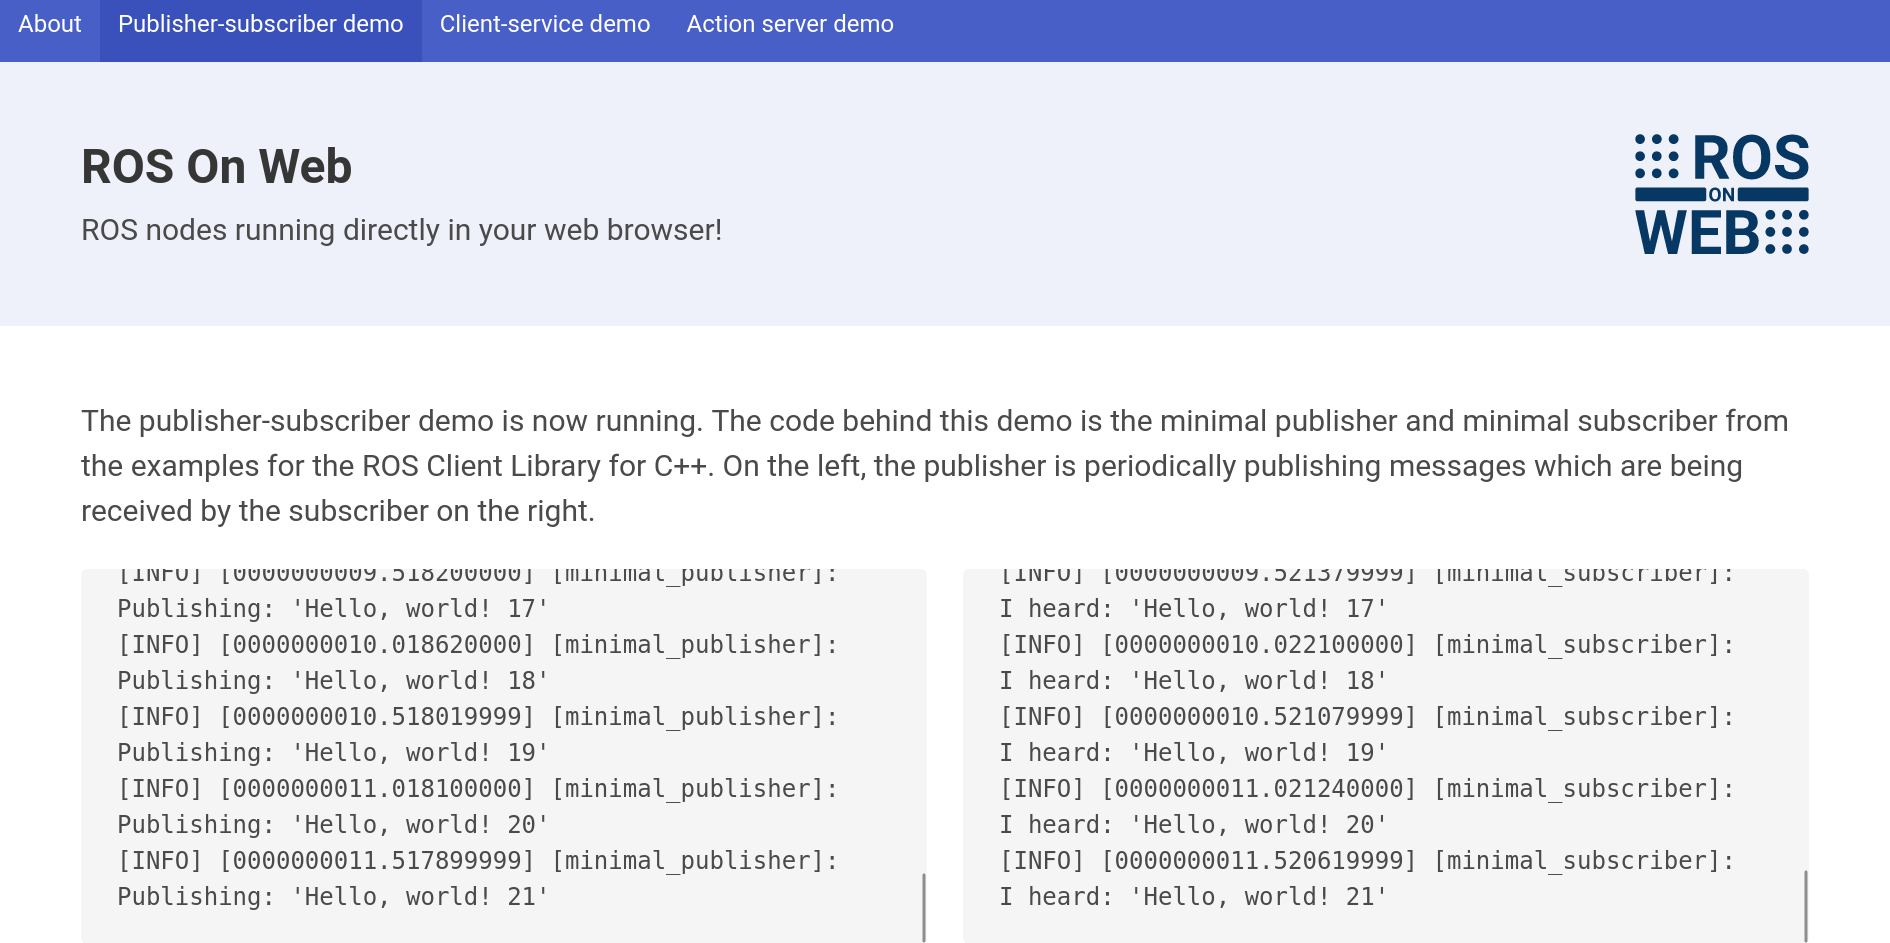
\includegraphics[width=\textwidth]{02_rosOnWeb.png}
            \caption{\textit{ROS on Web} publisher and subscriber demonstration.}
            \label{fig:rosonweb}
        \end{figure}

        Nonetheless, the greatest disadvantage of \textit{ROS on Web} lies in the fact that the project is not open source. Very little can be derived about how Allwright was able to achieve the demonstrations represented on the website. A few hints are given in the introductory page such as the replacement of the middleware with a custom design and the use of web workers. However, it is not possible to determine the manner in which these technologies were used. Hope remains that in the near future, the repositories for \textit{ROS on Web} become publicly available as an extension of the ROS open source ecosystem.

    \subsection{roswasm\_suite}

        Another project closely related to the author's developments is \textsf{roswasm\_suite} currently maintained mainly by Nils Bore. This suite is a set of libraries which help the user to cross\-compile C++ ROS nodes to WebAssembly~\cite{roswasmsuite}. It also includes a library of helpers to write web \ac{GUI}s for ROS; one such example can be observed in Figure~\ref{fig:roswasm_gui}.

        \begin{figure}[htbp]
            \centering
            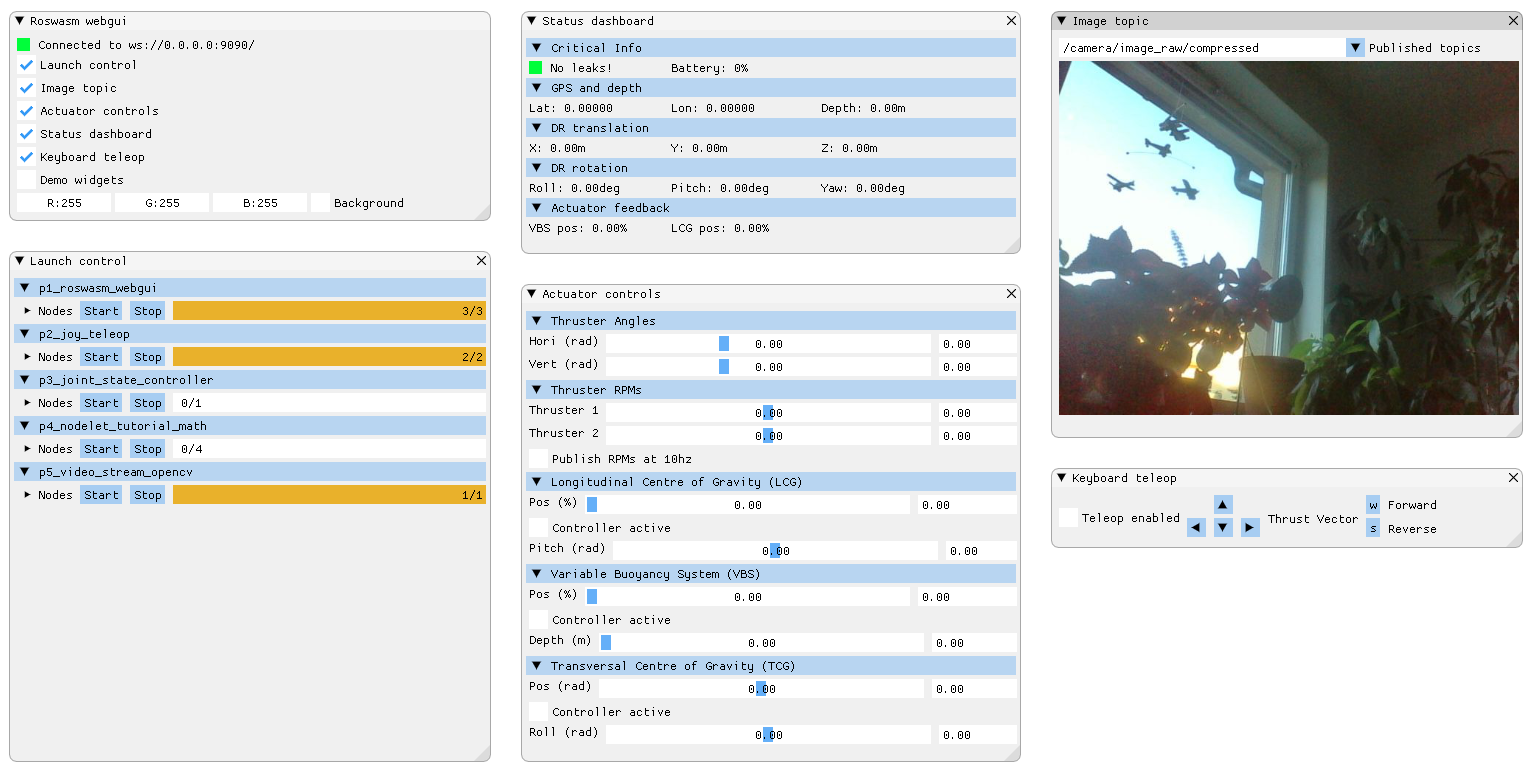
\includegraphics[width=\textwidth]{02_roswasm_gui.png}
            \caption{Example \ac{GUI} for ROS using \textsf{roswasm\_gui}.}
            \label{fig:roswasm_gui}
        \end{figure}

        Some of the biggest advantages of this \textsf{roswasm\_suite} are that it is open source and actively maintained. The developers have a long history of continuous improvements to the packages, and as of 2023, they have managed to publish ten releases. 

        Nevertheless, these libraries do come with their set of disadvantages. First, the suite targets a \ac{ROS} 1 distro and it depends on \textsf{catkin} tools to build the packages. Thus, the user is required to have a \ac{ROS} 1 installation and the Emscripten \ac{SDK} before being able to use these libraries to launch \ac{ROS} nodes on the browser.


\section{Relevant Works}

    There are several other works which do not directly align with the goals for this project but are pertinent in regards to the idea of developing a robotics environment which can be used on a web browser. Robot Web Tools maintains a collection of open source libraries and tools which can be used for robotic frameworks on the web~\cite{robotwebtools}.
    
    \subsection{Foxglove Studio}

        One of the most notorious examples of robotics applications on the browser consists of Foxglove Studio. The main focus of Foxglove Studio is visualization and debugging of robotic tasks~\cite{foxglove}. Given that their products are based on observability and not on direct control of robotic systems, this allows them to expand their service area to a wider range of systems and platforms. For example, Foxglove Studio supports both \ac{ROS} 1 and \ac{ROS} 2 distributions and the application can be installed on Linux, Windows and MacOS or run directly in Google Chrome.
        
        % https://foxglove.dev/blog/publishing-and-visualizing-ros2-transforms
        \begin{figure}[htbp]
            \centering
            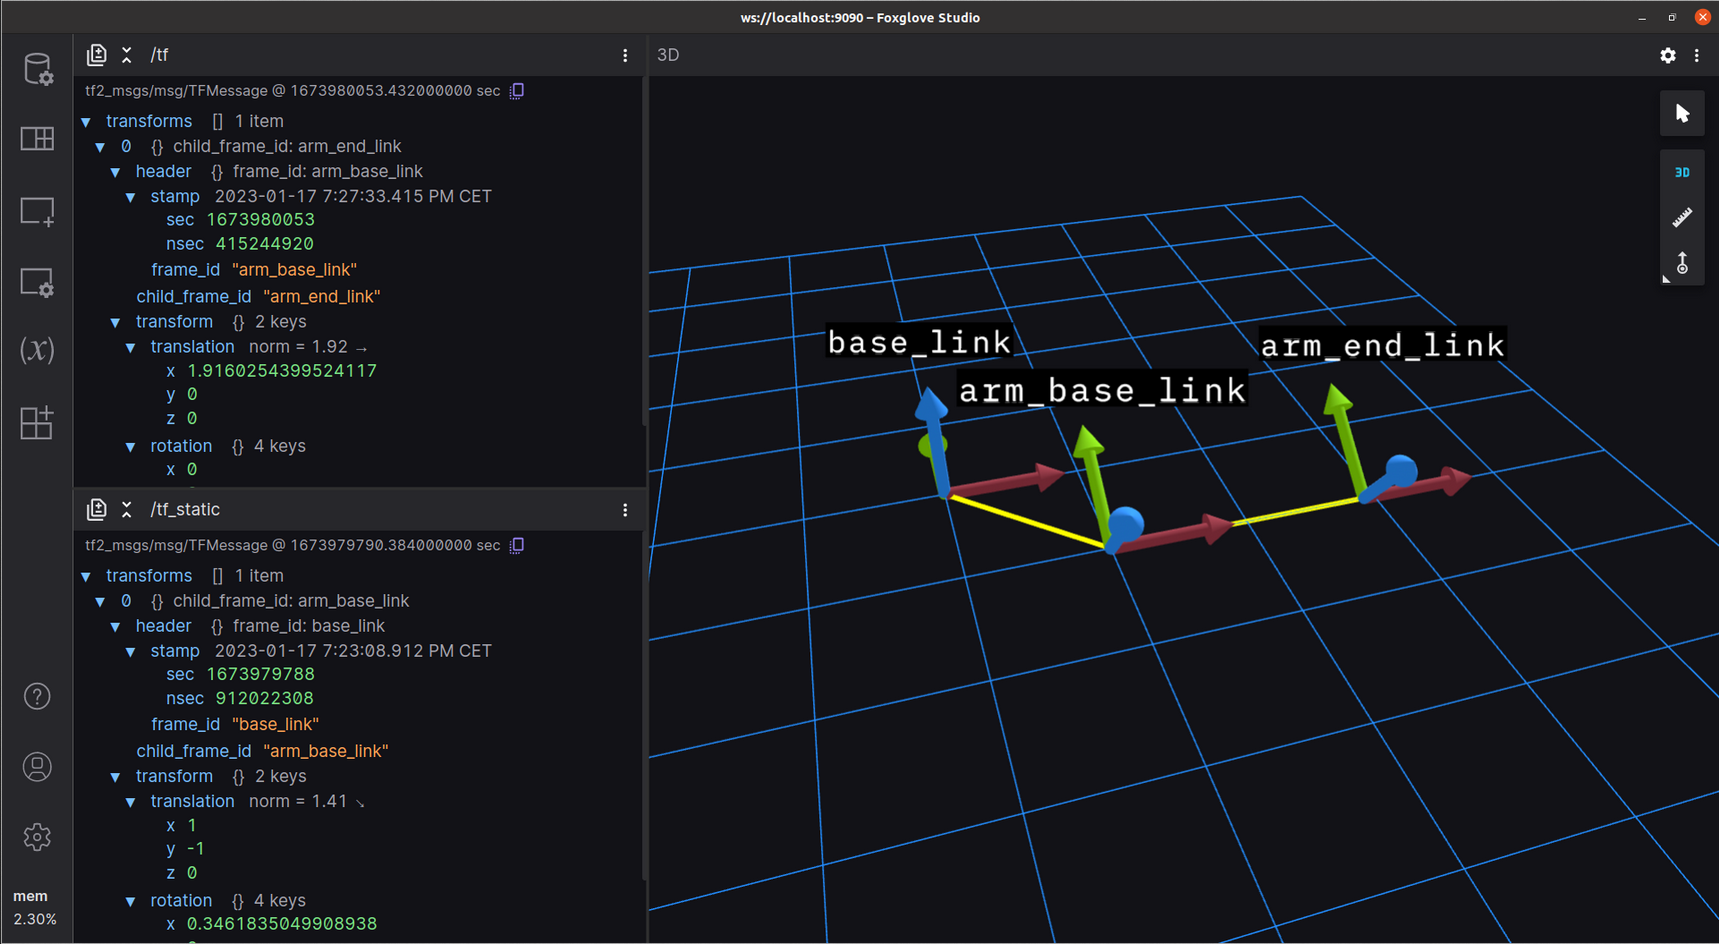
\includegraphics[width=\textwidth]{02_FoxgloveStudio.png}
            \caption{Visualizing ROS 2 Transforms with Foxglove Studio~\cite{transforms}.}
            \label{fig:foxglove}
        \end{figure}

        The wide range of visualization panels is one of the greatest strengths of Foxglove Studio. An example of a panel is shown in Figure~\ref{fig:foxglove} where \ac{ROS} 2 transforms are drawn in a graphical display. Additional examples of panels include support for visualizing raw messages, image topics, plots, parameters, \ac{URDF} models, etc.

        Another advantage of Foxglove Studio is that it is open source and actively maintained by community members. The application is also highly extensible with plugins to fit any specific needs of the users. Nevertheless, as a side effect of concentrating on observability, the application works as an add-on to an existing ROS installation and not as a replacement.

    \subsection{\textsf{rosbridge\_suite}}

        On a similar note, the \textsf{rosbridge\_suite} provides a set of packages which allow the user to interact with a \ac{ROS} system via a \ac{JSON} interface~\cite{rosbridge}. Hypothetically, with these libraries, any non-ROS systems could interact with ROS by sending \ac{JSON} messages. An instance of the \textsf{rosbridge} protocol can be seen in Figure~\ref{fig:rosbridge}.

        \begin{figure}[htbp]
            \centering
            \begin{lstlisting}[language=JSON]

  {
      "op": "subscribe",
      (optional) "id": <string>,
      "topic": "/cmd_vel",
      "type": "geometry_msgs/Twist"
  }
            \end{lstlisting}
            \caption{Example of \textsf{rosbridge} protocol emphasizing the JSON format.}
            \label{fig:rosbridge}
        \end{figure}

        The \textsf{rosbridge\_suite} consists of four main packages:

        \begin{itemize}
            \item \textsf{rosbridge\_suite}
            \item \textsf{rosbridge\_library}
            \item \textsf{rosbridge\_server}
            \item \textsf{rosapi}
        \end{itemize}

        From these packages, the \textsf{rosbridge\_library} performs the conversions from \ac{JSON} to \ac{ROS} messages and vice versa. While the \textsf{rosbridge\_server} provides the browsers with a WebSocket connection. A handful of \ac{API}s enable clients to communicate with \textsf{rosbridge}; these \ac{API}s are implemented in JavaScript, Java, Python, and Rust.

        Analogous to Foxglove Studio, \textsf{rosbridge} relies on an existing ROS installation. However, the capabilities of \textsf{rosbridge} are extensive and can be applied to real world scenarios; it also supports \ac{ROS} 1 and \ac{ROS} 2 distributions. Additionally, the community of contributors is highly involved in the maintenance of the client libraries.

    \subsection{ROS Control Center}\label{sec:roscontrolcenter}

        The \ac{ROS} Control Center is another web application which uses the \textsf{rosbridge\_suite} to establish a WebSocket connection to a robotics system running \ac{ROS}~\cite{controlcenter}. A view of the control center is depicted in Figure~\ref{fig:roscontrolcenter}.

        \begin{figure}[htbp]
            \centering
            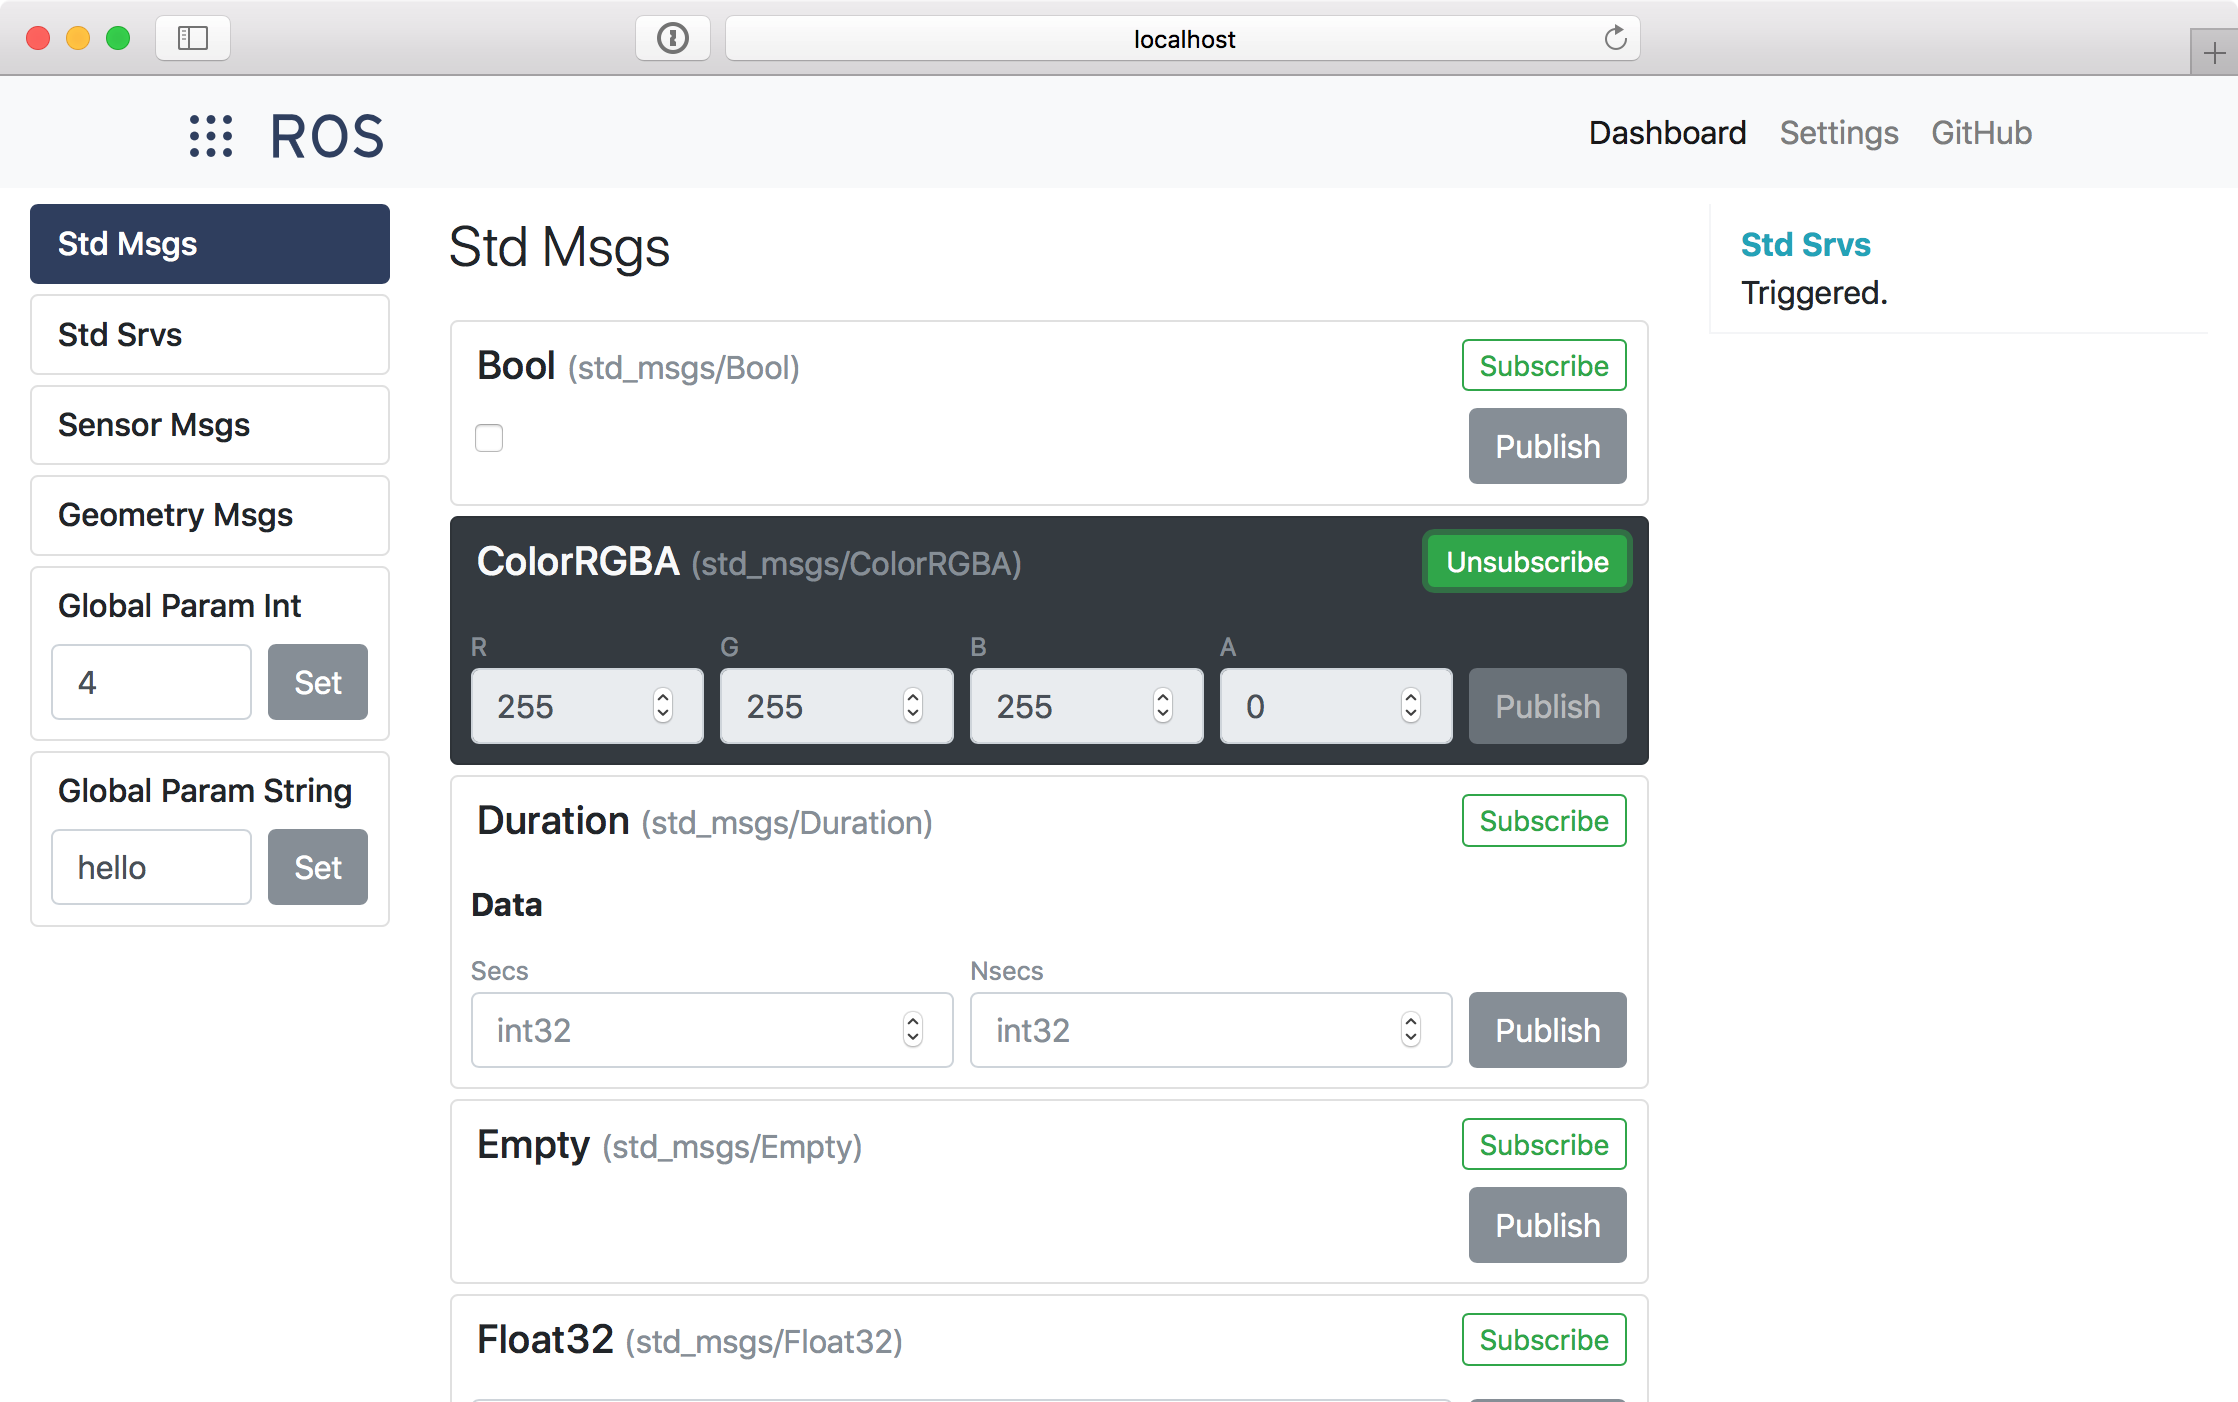
\includegraphics[width=\linewidth]{02_roscontrolcenter.png}
            \caption{ROS control center running locally.}
            \label{fig:roscontrolcenter}
        \end{figure}

        With this \ac{ROS} Control Center, the user is able to display information about running nodes, publish and subscribe to topics, call services, and change \ac{ROS} parameters. Despite its potential, the control center does not offer explicit support for interacting with \ac{ROS} 2 systems.

    \subsection{ROSWeb}

        ROSWeb combines all of the \ac{ROS} widgets collected by Robot Web Tools into a single web application~\cite{rosweb}. As in the case of~\ref{sec:roscontrolcenter}, ROSWeb also depends on \textsf{rosbridge} to interact with \ac{ROS} systems. Figure~\ref{fig:rosweb} demonstrates the ROSWeb application running on a Windows platform and communicating with a \ac{ROS} system in a virtual machine running Ubuntu.

        \begin{figure}[htbp]
            \centering
            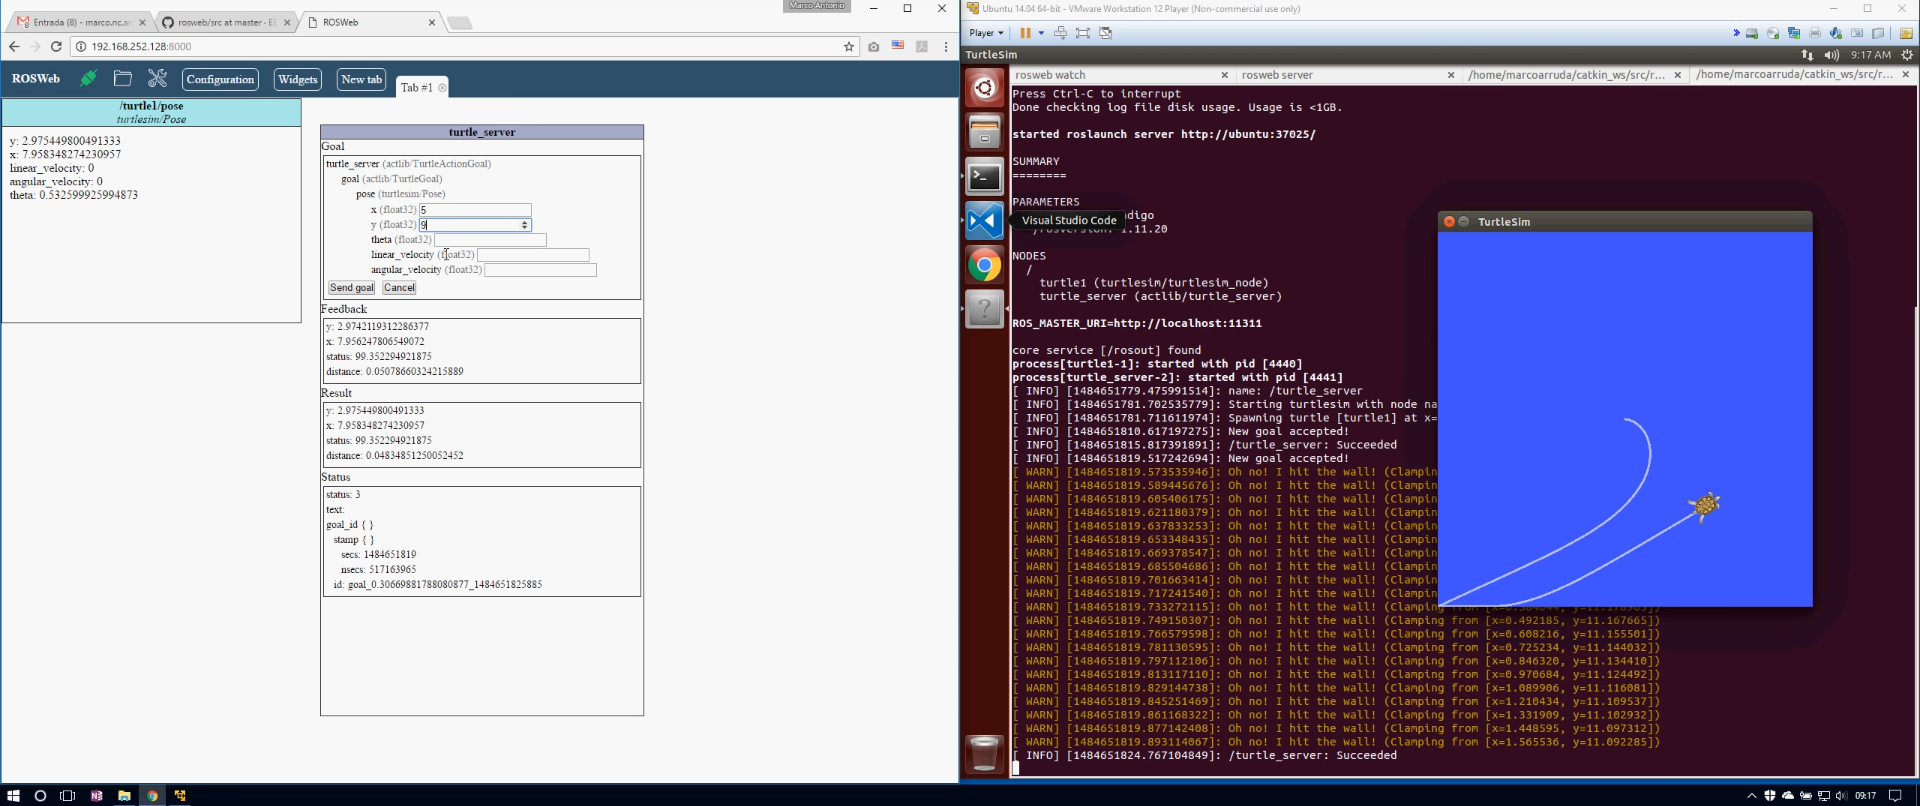
\includegraphics[width=\linewidth]{02_rosweb.png}
            \caption{ROSWeb application interacting with a \ac{VM} running \ac{ROS}.}
            \label{fig:rosweb}
        \end{figure}

        A major advantage of ROSWeb application is its simplicity. The \ac{ROS} widgets are interactive and require minimal programming experience from the users. It also enables the users to easily save and modify workspaces to match their needs.

    \subsection{ROSboard}

        In contrast to the previous two models, ROSboard does not rely on \textsf{rosbridge\_suite} to interact with \ac{ROS} systems; instead, it has a custom \textsf{Tornado} implementation to function as a web server and WebSocket server~\cite{rosboard}. Figure~\ref{fig:rosboard} shows and example of the ROSboard application with different visualization widgets.

        \begin{figure}[htbp]
            \centering
            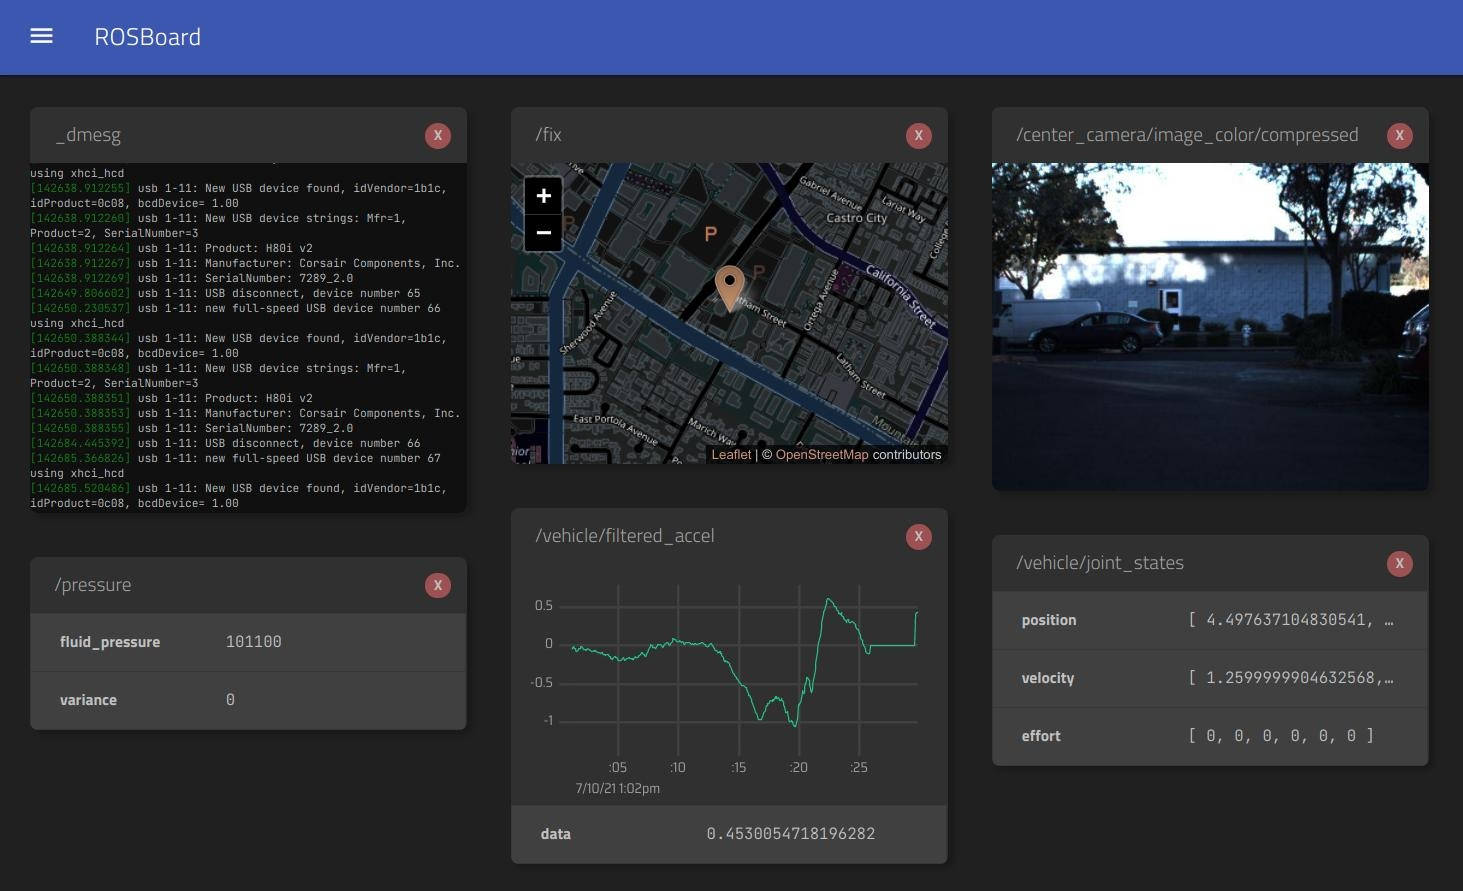
\includegraphics[width=\linewidth]{02_rosboard.jpg}
            \caption{ROSboard application visualizing multiple message types.}
            \label{fig:rosboard}
        \end{figure}

        ROSboard offers support for both \ac{ROS} 1 and \ac{ROS} 2 systems thanks to its tailored \textsf{rospy2} library which is based on \ac{ROS} 1's \textsf{rospy} but modified to ensure compatibility.

    \subsection{ROSLink}

    TODO: maybe too old to be relevant

\section{WebAssembly}

    TODO: describe what it is

    \subsection{A Brief History of WebAssembly}

        WebAssembly, also commonly referred to as simply WASM, is one of the newer technologies to 

    % https://blog.unity.com/technology/webassembly-is-here
    % https://beta.unity3d.com/jonas/AngryBots/

    \subsection{Applications}

    \begin{figure}[htbp]
        \centering
        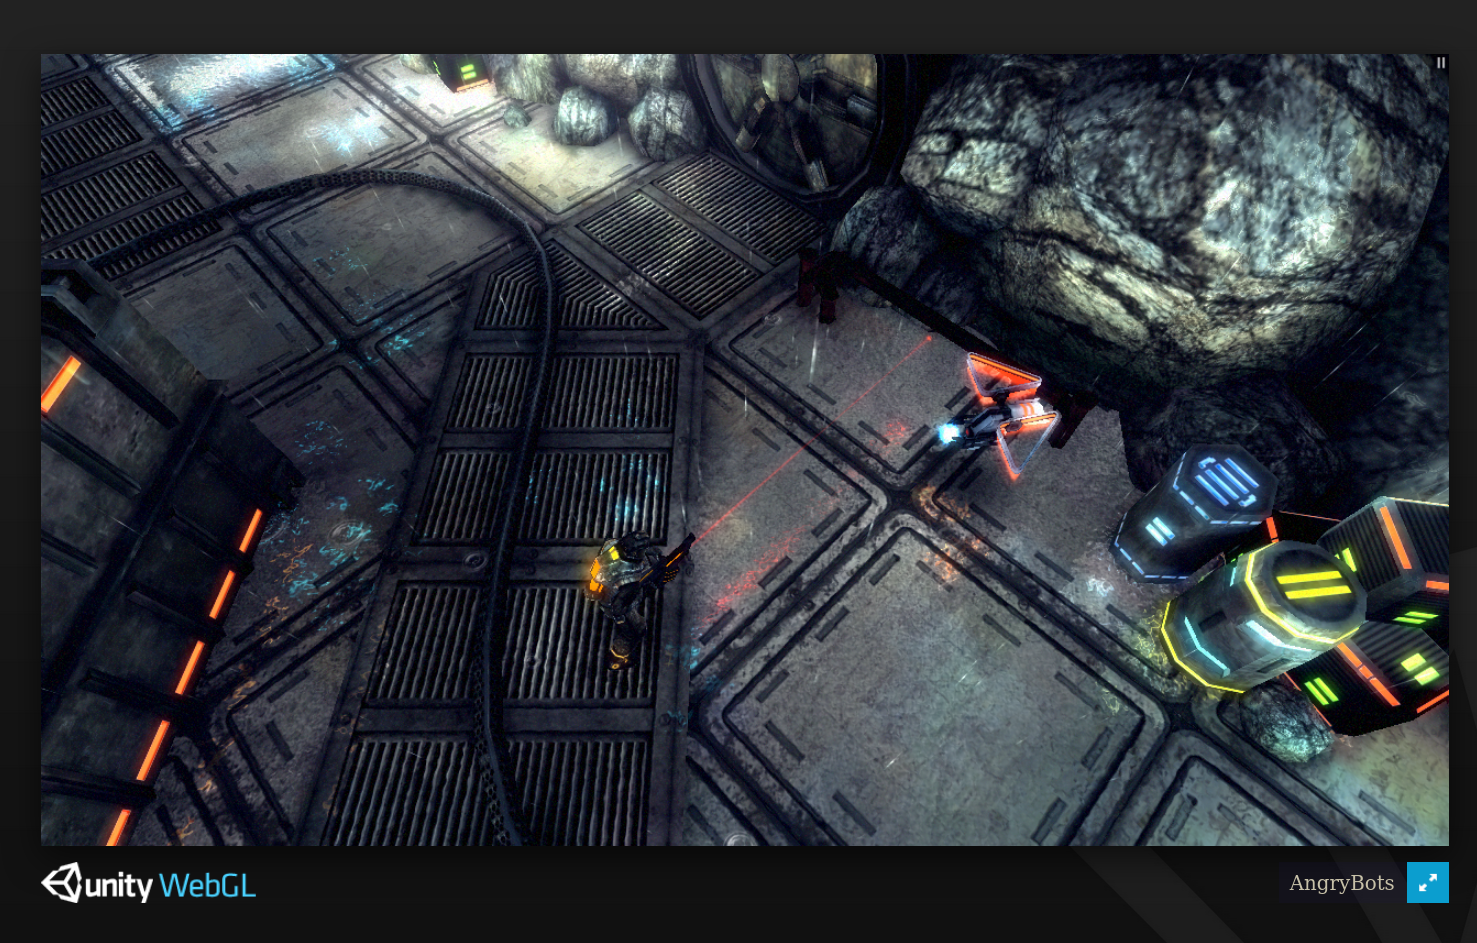
\includegraphics[width=\linewidth]{02_angryBots.png}
        \caption{Demo of Angry Bots in Unity WebGL}\label{fig:unity}
    \end{figure}


    \begin{figure}[htbp]
        \centering
        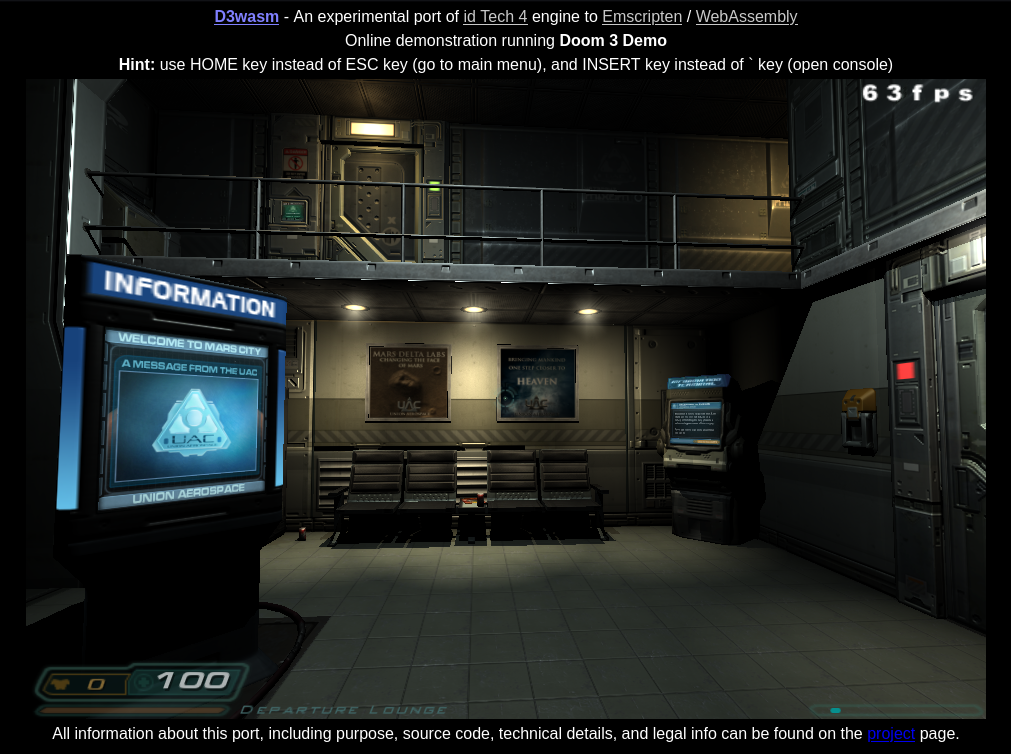
\includegraphics[width=\linewidth]{02_doom.png}
        \caption{Online demonstration of the \ac{D3wasm} project.}
        \label{fig:doom}
    \end{figure}


    \begin{figure}[htbp]
        \centering
        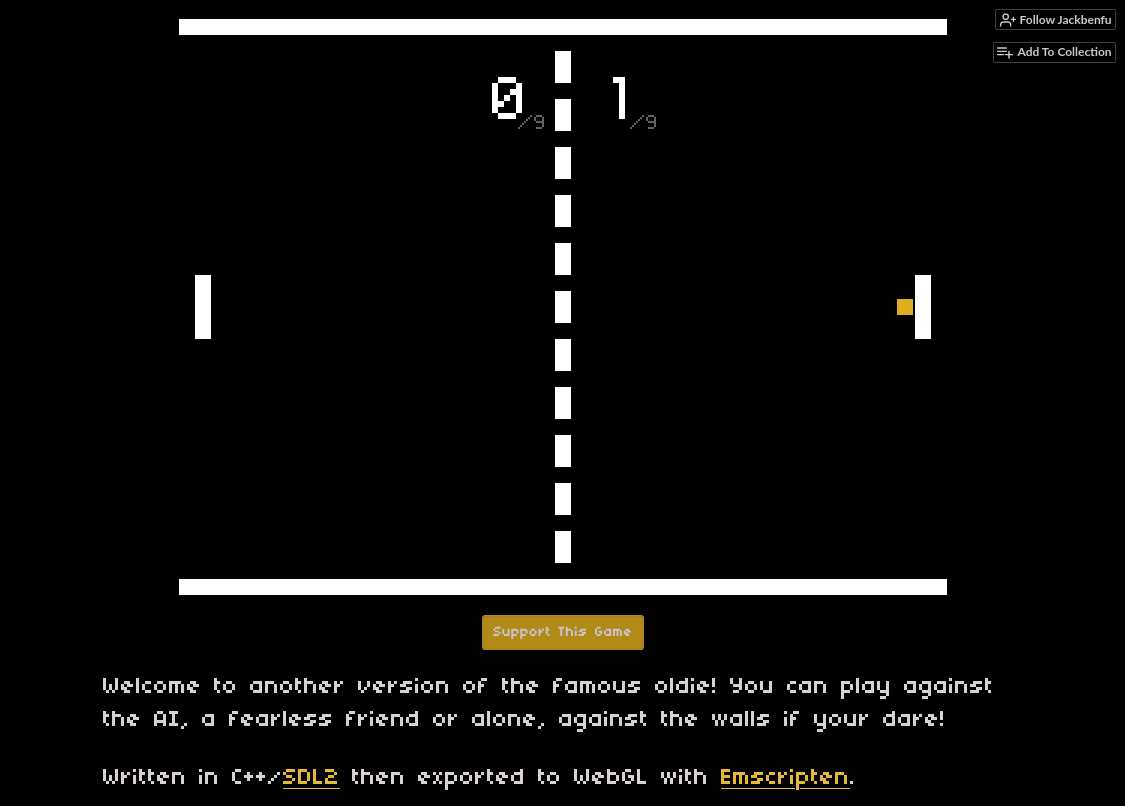
\includegraphics[width=\linewidth]{02_pong.png}
        \caption{TODO:}
        \label{fig:pong}
    \end{figure}

    \begin{figure}[htbp]
        \centering
        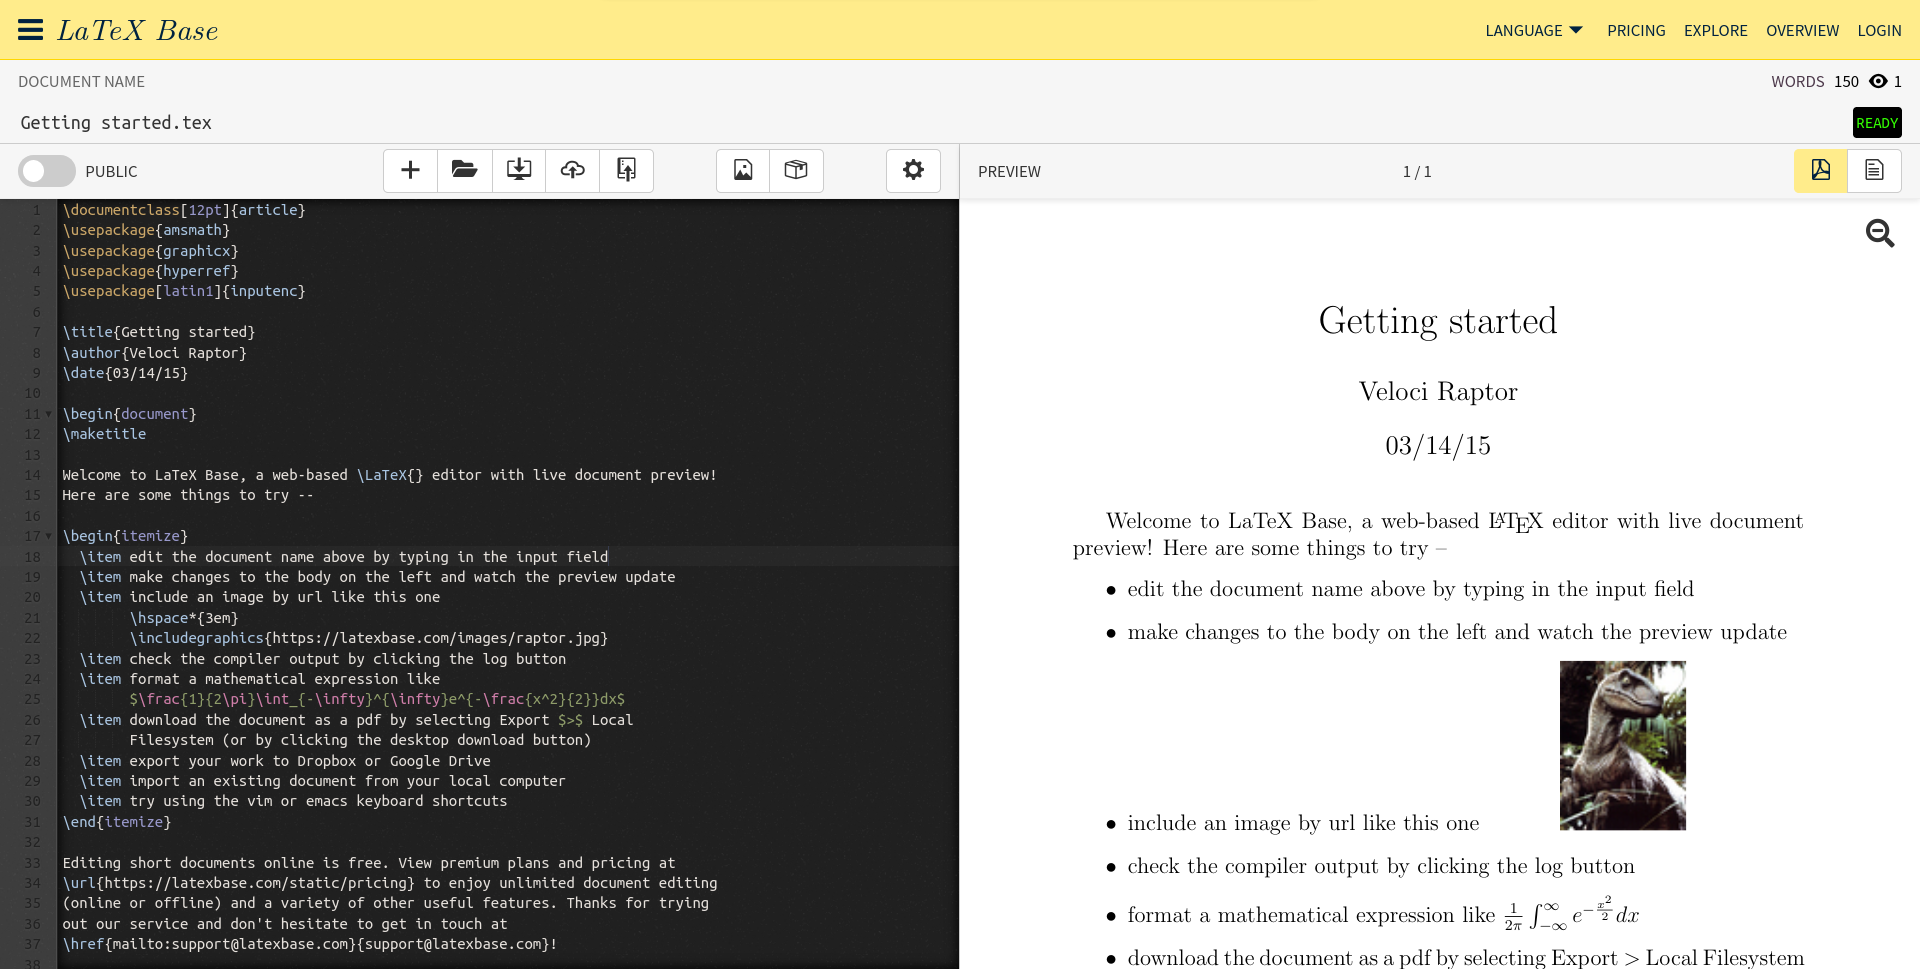
\includegraphics[width=\linewidth]{02_latexBase.png}
        \caption{TODO:}
        \label{fig:latex}
    \end{figure}
